
\documentclass[11pt,a4paper]{article}

\usepackage[utf8]{inputenc} 
\usepackage[T1]{fontenc} 
\usepackage{lmodern}
\usepackage{tcolorbox}
\usepackage[german]{babel}


\setlength{\parindent}{0pt}
\setlength{\parskip}{1ex plus 0.5ex minus 0.5ex}

\usepackage{amsmath} 


\usepackage{graphicx} 

\usepackage[section]{placeins}
\usepackage{booktabs}


\usepackage{hyperref}
\hypersetup{
	colorlinks,
	citecolor=red,
	filecolor=black,
	linkcolor=black,
	urlcolor=black}
\graphicspath{}

\begin{document}
	

{
	\centering 
	\large 
	Physiklabor für Anfänger*innen \\
	Ferienpraktikum im Sommersemester 2018 \\[4mm]
	\textbf{\LARGE 
		Versuch 70: Linsen und Linsensysteme
	} \\[3mm]
	(durchgeführt am 28.09.2018 bei Daniel Bartle) \\
	Ye Joon Kim, Marouan Zouari\\
	\today \\[10mm]
}
\tableofcontents
\newpage
\section{Einleitung}
Mit einer Linse kann man durch die Brechung Licht ablenken. Jede (richtig hergestellte) Linse besitzen zwei Brennpunkte, wo alle parallelen und zur Linse senkrecht einfallenden Lichtstrahlen sich sammeln. Der Abstand von dem Mittelpunkt der Linse zu einem Brennpunkt heißt die Brennweite. Für dicke Linsen und Linsensysteme muss einen weiteren Begriff eingeführt werden. Die doppelte Brechung lassen sich durch Hauptebenen beschreiben. Zwischen den Hauptebenen können die Lichtstrahlen als parallel verlaufend gedacht. Diese Begriffe vereinfachen Berechnungen mit Lichtstrahlen. 

Es existieren mehrere Verfahren, um die Brennweite von Linsen und Linsensysteme zu bestimmen. Bei einer Einzellinse kann die Brennweite $f$ so ausgedruckt werden: 

\begin{equation}
\frac{1}{f} = \frac{1}{g} + \frac{1}{b}
\end{equation}
Wobei $g$ und $b$ die Gegenstandsweite bzw. Bildweite, die Abstände von jeweils dem Gegenstand und Bild zur Linsenmitte, sind.
Für ein Linsensystem, das aus zwei Linsen besteht, gilt eine andere Formel, nämlich:
\begin{equation}
\frac{1}{f} = \frac{1}{f_1}+\frac{1}{f_2}-\frac{d}{f_1f_2}
\end{equation}
Wobei $f_1$ und $f_2$ die Brennweiten der einzelnen Linsen und $d$ der Abstand dazwischen sind. 

Aber wenn die Hauptebenen nicht bekannt sind, können $g$ und $b$ nicht direkt bestimmt werden. In diesem Fall hilft das Bessel-Verfahren, wobei die Brennweite mit:
\begin{equation}
f = \frac{s^2-e^2}{4s}
\end{equation}
bestimmt werden kann, wobei $s$ der Abstand zwischen dem Gegenstand und Bild, und $e$ die Differenz der Positionen, wo Abbildungen möglich sind. 

Mit einem anderen Verfahren, lassen sich die Brennweite und die Hauptebenen gleichzeitig bestimmen, dieses Verfahren heißt das Abbe-Verfahren. Hier zusätzlich zu die Werte der scheinbare Gegenstandweite und der scheinbare Bildweite wird  der Abbildungsmaßstab verwendet: 
$$ \beta = \frac{B}{G} = \frac{b}{g}$$
Wobei $B$ und $G$ jeweils die Größen des Bildes und Gegenstands sind. 
Mit direkten Messungen von $B$, $G$, $g'$ ( die scheinbare Gegenstandweite) und $b'$ (die scheinbare Bildweite) kann mit den Gleichungen:
\begin{equation}
\begin{array}{l}
	g' = (1+\frac{1}{\beta})\cdot f_1 + h_1 \\
	b' = (1+\beta)\cdot f_2 + h_2
\end{array}
\end{equation}
die $f$ und $h$ bestimmt werden, da $f$ die Steigungen, und $h$ den Achsenabschnitte entsprechen. 



\section{Aufbau}
\begin{figure}[h]
	\centering
	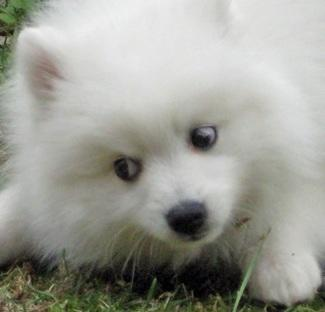
\includegraphics[scale=1]{ver70}
	\caption{Versuchsaufbau}
\end{figure}
Zu diesem Versuch wurden ein Schirm, ein Dia, mehrere Linsen, eine Linsenhalterung, ein Spiegel, eine Lichtquelle und eine optische Bank benutzt. 

\section{Durchf"uhrung}
Damit das Licht parallel zur optischen Bank verläuft, wurde zuerst eine Kollimationslinse direkt vor der Lichtquelle eingesetzt. Der Schirm wurde auf der anderen Seite der Bank fixiert, sodass eine relativ scharfe Abbildung zu sehen war. Die Abbildung wurde dann mit den Drehknöpfen auf der Lichtquelle zentriert. 

Für den ersten Versuchsteil wurde das Dia hinter der Kollimationslinse eingesetzt und durch das Verschieben der Linsenhalterung wurde das Dia seitenverkehrt und scharf auf den Schirm abgebildet.
Die Positionen der Linsenhalterung, Dia und Schirm wurden mithilfe der Skala auf der optischen Bank gemessen. Dies wurde für fünf unterschiedliche Positionen des Schirms wiederholt, und der gesamte Prozess wurde für drei verschiedene Linse und Linsensysteme wiederholt. 
\\\
Für den zweiten Versuchsteil wurden die in dem ersten Teil gemessenen Daten verwendet, deswegen wurde keine neuen Messungen durchgeführt. 
\\\
Bei der dritten Teil wurde das Abbe-Verfahren benutzt, um die Brennweite und Lage der Hauptebenen zu bestimmen. Für diesen Teil wurde ein Linsensystem mit einer $f=$ 80mm Sammellinse und einer $f=$ -200mm Zerstreuungslinse benutzt. Ähnlich wie in dem ersten Teil, wurde die Linsenhalterung so verschoben, sodass eine scharfe Abbildung der Dia auf dem Schirm entstanden war. Die Positionen des Schirms und der Linsenhalterung wurden dann gemessen. Mit einem Lineal wurde der Durchmesser von einer der auf den Schirm abgebildeten Kreise gemessen. Diese Schritte wurden dann für 10 unterschiedliche Positionen des Schirms wiederholt und der gesamte Prozess für umgekehrte Reihenfolge der Linsen wiederholt. 

In dem letzten Versuchsteil wurde die Brennweite mithilfe des Autokollimationsverfahrens bestimmt. Dafür wurde der Spiegel nah hinter der Linse gesetzt und justiert, sodass das reflektierte Bild ein Bisschen oben versetzt entsteht. Die Linse und Spiegel wurden zusammen verschoben, sodass das Dia auf den Diarahmen scharf abgebildet wird. Die Lage der Linse wurde dann gemessen. Dieser Prozess wurde für verschiedene Linse, Linsensysteme und Lichtfarben wiederholt.

\section{Auswertung und Fehleranalyse}
\subsection{1. Versuchsteil: Abbildungen mit Einzellinsen und Linsensystemen}
Die Werte für $\frac{1}{b}$ wurden gegen $\frac{1}{g}$ aufgetragen. Für jede Messreihe wurde auch lineare Regressionen durchgeführt, aber nur, um die Linearität der Zusammenhang zu veranschaulichen (Siehe Abbildung 1). Die theoretische Verläufe wurden auch mit Formel (2) und (1) berechnet (Siehe Abbildung 2). 
\begin{figure}
	\centering
	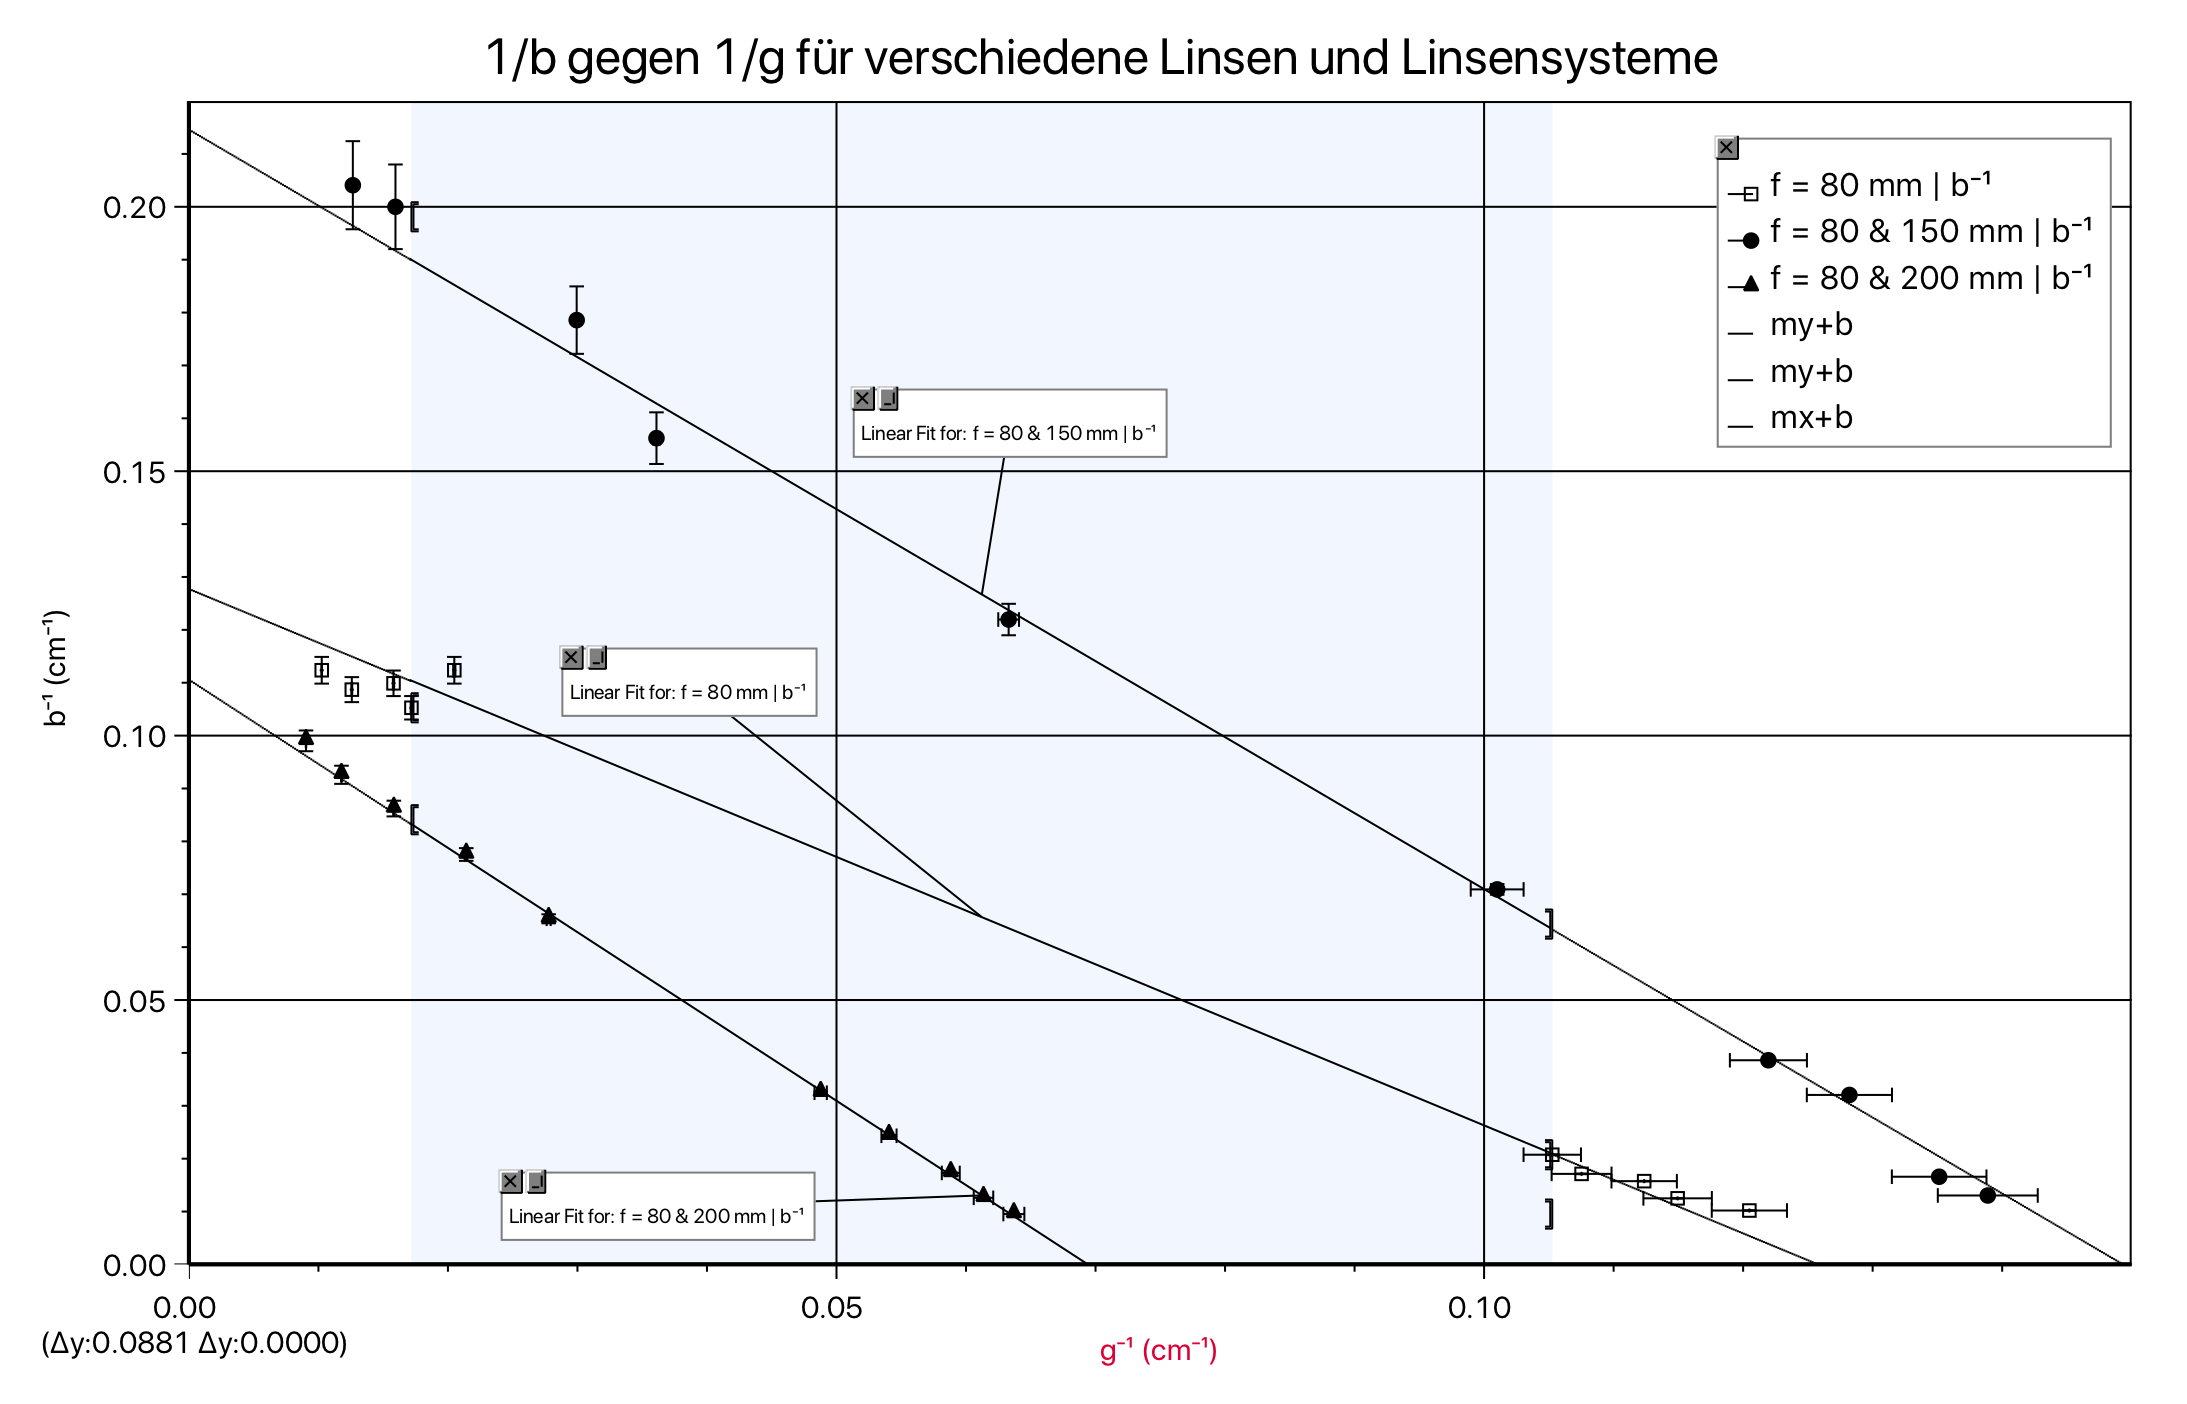
\includegraphics[width=\linewidth]{Abb2}
	\caption{$\frac{1}{b}$ gegen $\frac{1}{g}$.}
\end{figure} 

\begin{figure}
	\centering
	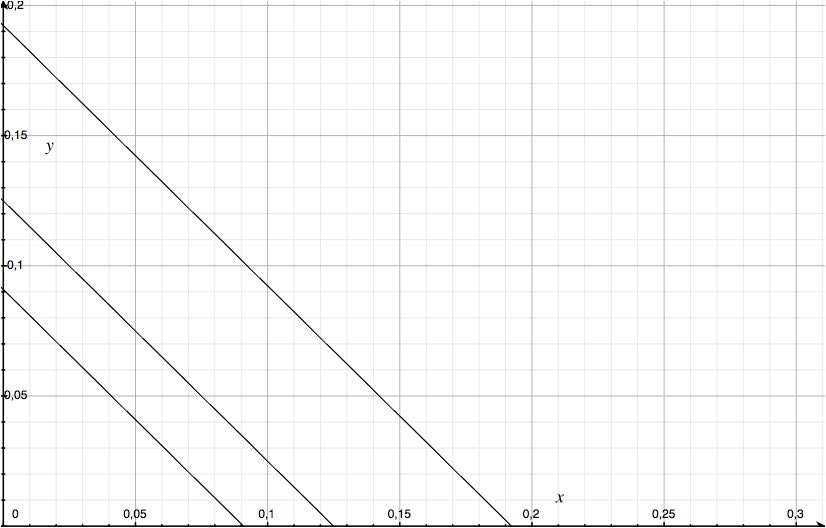
\includegraphics[scale=0.5]{Abb3}
	\caption{ Die aus der Abbildungsgleichung Erwarteten Linearen Verläufe}
\end{figure} 

\begin{tcolorbox}[colback=white]
\subsubsection{Rechenweg}
Zuerst wurde die Unsicherheiten von $g$ und $b$ mit der vereinfachten gauß'schen Fehlerfortpflanzung für Summe berechnet. Zum Beispiel:
$$ \Delta g = \sqrt{(\Delta x_\textrm{Dia})^2 + (\Delta x_\textrm{Groß})^2}$$
, da $g = x_\textrm{Groß} - x_\textrm{Dia}$, wobei $x_\textrm{Dia}$ die Position des Dias und $x_\textrm{Groß}$ die Position der Linse, wo eine vergrößernde Abbildung möglich ist. 

Die Unsicherheiten der einzelnen Punkten auf der Graph wurde mit der vereinfachten gaußschen Fehlerfortpflanzung für Produkte und Quotienten bestimmt.
$$ \Delta\left(\frac{1}{g}\right) = \frac{\Delta g}{g} \cdot \frac{1}{g}$$
ebenfalls für die $\frac{1}{b}$ Werte. 
	
Für die theoretischen Verläufe wurde Gleichung (1) nach $\frac{1}{b}$ umgeformt und die gesamten Brennweiten mit Gleichung (2) Berechnet. 
	
	
\end{tcolorbox}

\subsection{2. Versuchsteil: Das Bessel-Verfahren}
Gemäß Gleichung (3) wurden die Werte für $s$ und $e$ und deren Unsicherheiten berechnet (Siehe Anhang 1). Die Unsicherheiten wurde wie in dem ersten Versuchsteil mit der gauß'sche Fehlerfortpflanzung für Summe berechnet. Danach wurden die einzelne Werte für $f$ für jede Messreihe berechnet (Siehe Anhang 2). 

Die Unsicherheiten der $f$ Werte wurden mit der gauß'schen Fehlerfortpflanzung berechnet. Mit 
$$ f = \frac{s^2-e^2}{4s}$$
sind:
$$ \frac{\partial f}{\partial{s}} = \frac{s^2+e^2}{4s^2}$$
$$\frac{\partial f}{\partial{e}} = -\frac{e}{2s}$$
Die Unsicherheit von $f$ ist deshalb:
$$\Delta f = \sqrt{(\frac{\partial f}{\partial{s}}\Delta s)^2 + (\frac{\partial f}{\partial{e}} \Delta e)^2}$$

Die Mittelwerte der $f$ für jede Linse/Linsensystem und deren Standardunsicherheiten sind dann:

\begin{table} [h]
	\centering
	\begin{tabular*}{0.50\textwidth}{@{\extracolsep{\fill}}c|cccccc}
		\toprule
		Brennweite & $f$ & $u_f$   \\
		mm & cm & cm \\
		\bottomrule
		80 & 7,93 & 0,06 \\
		80 \& 150 & 5,63 & 0,03 \\
		80 \& -200 & 11,59 & 0,02 \\
		\bottomrule
	\end{tabular*}
	\caption{Die Berechneten $f$ für die Linsen und Linsensysteme}
\end{table}

\begin{tcolorbox}[colback=white]
	\subsubsection{Rechenweg}
	Zur Bestimmung der Standardunsicherheiten wurden zuerst die Standardabweichung berechnet mit der folgenden Formel:
	$$s_x = \sqrt{\frac{\sum_{i=1}^{n}(x_i-\bar{x})^2}{n-1}} $$
	
	Da die $f$ Werte Mittelwerte sind wurde diese Standardabweichung mit einem Faktor $\sqrt(m)$ geteilt. Die Unsicherheit ist deshalb:
	$$u_x = \frac{s_x}{\sqrt{n}}$$
\end{tcolorbox}

\subsection{3. Versuchsteil: Das Abbe-Verfahren}
Zuerst wurden die Werte für $\beta$ ausgerechnet (Siehe Tabelle 1).



\begin{table}[h]
	\centering
	\begin{tabular*}{0.50\textwidth}{@{\extracolsep{\fill}}cc|ccccc}
		\toprule
		$g'$ & $b'$ & $\beta$ & $\Delta \beta$   \\
		cm & cm& &\\
		18,5&47,9&3,33&0,05\\
		20,8&28,6&1,71&0,05\\
		19,7&25,0&2,19&0,05\\
		17,8&47,2&3,71&0,05\\
		15,3&74,7&4,71&0,14\\
		16,1&90,3&6,71&0,14\\
		16,0&101,8&7,86&0,14\\
		17,3&54,6&3,79&0,07\\
		18,3&41,7&2,71&0,07\\
		18,4&39,0&2,57&0,14\\
		\bottomrule
	\end{tabular*}
	\caption{Die gemessenen Werte für $g'$, $b'$ und $\beta$ für ein Linsensystem mit $f_1 = 80mm$ und $f_2 = -200mm$}
\end{table}



\begin{table}[h]
	\centering
	\begin{tabular*}{0.50\textwidth}{@{\extracolsep{\fill}}cc|ccccc}
		\toprule
		$g'$ & $b'$ & $\beta$ & $\Delta \beta$   \\
		cm & cm& &\\
		13,5&58,6&2,86&0,14\\
		13,9&51,5&3,21&0,07\\
		14,6&44,3&2,64&0,07\\
		21,4&25,3&1,00&0,07\\
		12,4&93,6&6,86&0,14\\
		12,4&84,5&6,14&0,14\\
		12,0&108,6&8,14&0,14\\
		12,9&76,0&8,00&0,14\\
		12,8&68,6&4,64&0,07\\
		14,3&48,6&3,00&0,07\\
		\bottomrule
	\end{tabular*}
	\caption{Die gemessenen Werte für $g'$, $b'$ und $\beta$ für ein Linsensystem mit $f_1 = -200mm$ und $f_2 = 80mm$}
\end{table}

\FloatBarrier
Danach wurden $g'$ und $b'$ jeweils gegen $(1+\frac{1}{\beta})$ und $(1+\beta)$ aufgetragen (Siehe Anhang 3, 4). 
Dadurch lassen sich die Werte für $f_1$, $f_2$, $h_1$ und $h_2$ für beide Linsensysteme bestimmen. 
Das System mit zuerst einer Linse mit $f=80mm$ und danach einer mit $f=-200mm$ hat die folgenden Werte:
$$f_1 = 11\textrm{cm    } f_2 = 12\textrm{cm}$$
$$ h_1 = 3\textrm{cm    } h_2 = -8 \textrm{cm}$$

Und für das System mit umgekehrter Reihenfolge der Linsen:
$$f_1 = 3\textrm{cm    } f_2 = 10 \textrm{cm}$$
$$ h_1 = 10\textrm{cm    } h_2 = 18 \textrm{cm}$$


\subsection{4. Versuchsteil: Autokollimationsverfahren und Dispersion}
Der Abstand zwischen der Linse und dem Objekt, wobei eine Scharfe Abbildung möglich war, wurde für verschiedene Linsen und Linsensysteme und danach mit einer Linse mit verschiedenen Lichtfarben berechnet. Dieser Abstand entspricht dann der Brennweite. 


\begin{table}[h]
	\centering
	\begin{tabular*}{0.75\textwidth}{@{\extracolsep{\fill}}c|cc}
		\toprule
		Brennweite & $f$ & $\Delta f$ \\
		der einzelnen Linsen &&\\
		mm & cm & cm \\
		80  & 7,6 & 0,3 \\
		150 & 24,6 & 0,3 \\
		80 \& 150 & 4,6 & 0,3 \\
		80 \& -200 & 12,2 & 0,3 \\
		-200 \& 80 & 8,0 & 0,3\\
		\bottomrule
	\end{tabular*}
	\caption{Die mit dem Autokollimationsverfahren bestimmten $f$ für verschiedene Linsen und Linsensysteme.}
\end{table}

\begin{table}[h]
	\centering
	\begin{tabular*}{0.75\textwidth}{@{\extracolsep{\fill}}c|cc}
		\toprule
		Lichtfarbe & $f$ & $\Delta f$ \\
		 & cm & cm \\
		Weiß  & 33,6 & 0,3 \\
		Rot & 33,5 & 0,3 \\
		Blau & 32,8 & 0,3 \\
		\bottomrule
	\end{tabular*}
	\caption{Die mit dem Autokollimationsverfahren bestimmten $f$ für verschiedene Lichtfarben}
\end{table}

Zur Bestimmung der Unsicherheiten wurde die vereinfachte Fehlerfortpflanzung für Summe verwendet. Deswegen ist $\Delta f$:
$$\sqrt{2\cdot(0,2 \textrm{cm})^2} \approx 0,28$$


\subsection{Bestimmung der theoretischen Brennweiten}
Zur Bestimmung der theoretische Brennweiten der Verschiedene Linsensysteme wurde die folgende Formel benutzt (Formel 2):
$$
\frac{1}{f} = \frac{1}{f_1}+\frac{1}{f_2}-\frac{d}{f_1f_2}
$$

Wobei $d$ der Abstand zwischen den Linsen ist. 

Dadurch lassen sich die Gesamt-Brennweiten der Linsensysteme bestimmen. 

\begin{table}[h]
	\centering
	\begin{tabular*}{0.75\textwidth}{@{\extracolsep{\fill}}c|cc}
		\toprule
		Brennweite & $f_\textrm{tot}$  \\
		der einzelnen Linsen &\\
		mm & mm \\
		80 \& 150  & 48  \\
		80 \& -200 & 162 \\
		-200 \& 80 & 162 \\
		\bottomrule
	\end{tabular*}
	\caption{Die theoretische Gesamt-Brennweiten der in dem Versuch verwendeten Linsensysteme}
\end{table}

\section{Diskussion der Ergebnisse}
\subsection{Erster Versuchsteil}
(Siehe Abbildung 2) Es kann leicht von den Gleichungen gesehen werden, dass die linearen Regressionen theoretisch dieselbe Steigung haben müssen. Die lineare Regression für $f=$80mm hat aber eine bemerkbare schwächere Steigung als die anderen zwei Kurven. 

Der Achsenschnitt von zwei linearen Regressionen stimmen mit den theoretischen Verläufe überein. Für das Linsensystem mit der Zerstreuungslinse gab es eine Abweichung von 0,05 cm zwischen den extrapolierten  und theoretischen Achsenabschnitte, was fast 50\% des Wertes selbst beträgt. Möglicher Fehlerquellen werden später diskutiert. 

\subsection{Zweiter Versuchsteil: Das Bessel Verfahren}
Die mit dem Bessel-Verfahren bestimmte Brennweiten der Linsen und Linsensysteme sind:

\begin{table} [h]
	\centering
	\begin{tabular*}{0.50\textwidth}{@{\extracolsep{\fill}}c|cccccc}
		\toprule
		Brennweite & $f$ & $u_f$   \\
		mm & cm & cm \\
		\bottomrule
		80 & 7,93 & 0,06 \\
		80 \& 150 & 5,63 & 0,03 \\
		80 \& -200 & 11,59 & 0,02 \\
		\bottomrule
	\end{tabular*}
	\caption{Die mit dem Bessel-Verfahren berechneten $f$ für verschiedene Linsen und Linsensysteme}
\end{table}

Um zu sehen, ob die gemessenen Werte und die theoretischen Werte miteinander verträglich sind wurde ihre Differenzen in Einheiten der Standardunsicherheit berechnet. Mit der folgenden Formel:
$$ t = \frac{f-f_\textrm{theo}}{u_f}$$
sind:
$$ t_\textrm{80 mm} = 1,17$$
$$ t_\textrm{80 \& 150 mm} = 11,86$$
$$ t_\textrm{80 \& 200 mm} = 92,20$$
Da die Werte für $t_\textrm{80 \& 150 mm}$ und $t_\textrm{80 \& 200 mm}$ viel größer als 2 sind, sind diese Ergebnisse mit den theoretischen Werten nicht verträglich. Aber das impliziert nicht, dass diese Werte nicht plausibel sind. Die theoretischen Werte wurden gemäß den gegebenen Abmessungen der Linsenhalterung berechnet. Es gab aber auch eine andere Berechnung von einer anderen Person, die besagt, dass die theoretischen Brennweiten $f_\textrm{80 \& 150 mm}$ und $f_\textrm{80 \& -200 mm}$ jeweils ungefähr 5,2 cm und 11 cm sind. Diese theoretischen Werte sind viel näher an den gemessenen Werten (aber sie sind jedoch miteinander nicht verträglich). 

\subsection{Dritter Versuchsteil: Das Abbe-Verfahren}
Der für diesen Versuchsteil ausgewählte Referenzpunkt war die linke Seite der Linsenhalterung. $f_1$, $f_2$, $h_1$ und $h_2$ sind die Lagen der Brennpunkte und Hauptebenen relativ zu diesem Punkt. Die Brennweite und Abstand zwischen den Hauptebenen muss deshalb zweimal von jeweils $f_1-f_2$ und $h_1-h_2$ sein. Diese Werte müssen für beide Messreihen übereinstimmen. Die gemessenen Brennweite und Abstände zwischen den Hauptebenen sind:
$$ f = 0,5 \textrm{ cm und }  3,5 \textrm{ cm}$$
$$ h = 5,5 \textrm{ cm und } 4 \textrm{ cm} $$
Die Werte stimmen miteinander und mit der theoretischen Brennweite nicht überein. Es kann auch graphisch gesehen werden (Anhang 3,4) dass die Streuung der Punkte auch sehr groß ist. Diese Ergebnisse sind deshalb von keiner großen Bedeutung. 

\subsection{Vierter Versuchsteil: Das Autokollimationsverfahren}
Die mit dem Autokollimationsverfahren bestimmten Brennweiten sind in Tabelle 8 zu sehen. 


\begin{table}[h]
	\centering
	\begin{tabular*}{0.75\textwidth}{@{\extracolsep{\fill}}c|cc}
		\toprule
		Brennweite & $f$ & $\Delta f$ \\
		der einzelnen Linsen &&\\
		mm & cm & cm \\
		80  & 7,6 & 0,3 \\
		150 & 24,6 & 0,3 \\
		80 \& 150 & 4,6 & 0,3 \\
		80 \& -200 & 12,2 & 0,3 \\
		-200 \& 80 & 8,0 & 0,3\\
		\bottomrule
	\end{tabular*}
	\caption{Die mit dem Autokollimationsverfahren bestimmten $f$ für verschiedene Linsen und Linsensysteme.}
\end{table}

Die Differenzen zwischen den gemessenen Werten und den theoretischen Werten wurden erneut berechnet:
$$t_\textrm{80 mm} = 1,33$$
$$t_\textrm{150 mm} = 32$$
$$t_\textrm{80 \& 150 mm} = 3,33 $$
$$t_\textrm{80 \& -200 mm} = 13,33$$
$$t_\textrm{-200 \& 80 mm} = 27,33$$

Nur für $f=$ 80 mm waren die gemessenen und theoretischen Werte miteinander verträglich. Die anderen Ergebnisse sind absurd. 

\subsection{systematischen und statistischen Fehler}

\section{Anhang}


\begin{table}[h]
	\centering
	\begin{tabular*}{0.50\textwidth}{@{\extracolsep{\fill}}cc|ccccc}
		\toprule
		Brennweite & Messreihe & $s$ & $e$   \\
		mm &  & cm & cm  \\
		\bottomrule
		80 & 1 & 57,7 & 39,3 \\
		& 2 & 72,4 & 54,4 \\
		& 3 & 88,7 & 70,8 \\
		& 4 & 106,4 & 89,2 \\
		& 5 & 67,7 & 48,9 \\
		80 \& 150 & 1 & 67,7 & 55,3 \\
		& 2 & 83,9 & 71,8 \\
		& 3 & 34,1 & 19,5 \\
		& 4 & 24,0 & 5,9 \\
		& 5 & 39,0 & 25,6 \\
		80 \& -200 & 1 & 95,7 & 68,6 \\
		& 2 & 74,8 & 46,2 \\
		& 3 & 120,7 & 94,9 \\
		& 4 & 59,6 & 28,2 \\
		& 5 & 51,3 & 15,5 \\
		\bottomrule
	\end{tabular*}
	\caption{Die Werte für $s$ und $e$ für alle Messreihen}
\end{table}


\begin{table}[h]
	\centering
	\begin{tabular*}{0.50\textwidth}{@{\extracolsep{\fill}}cc|ccccc}
		\toprule
		Brennweite & Messreihe & $s$ & $e$   \\
		mm &  & cm & cm  \\
		\bottomrule
		80 & 1 & 7,73 & 0,14 \\
		& 2 & 7,88 & 0,15 \\
		& 3 & 8,05 & 0,16 \\
		& 4 & 7,90 & 0,17 \\
		& 5 & 8,09 & 0,15 \\
		80 \& 150 & 1 & 5,63 & 0,17 \\
		& 2 & 5,61 & 0,17 \\
		& 3 & 5,73 & 0,12 \\
		& 4 & 5,64 & 0,08 \\
		& 5 & 5,55 & 0,14 \\
		80 \& -200 & 1 & 11,63 &0,15 \\
		& 2 & 11,56 & 0,13 \\
		& 3 & 11,52 & 0,16 \\
		& 4 & 11,56 & 0,11 \\
		& 5 & 51,3 & 0,09 \\
		\bottomrule
	\end{tabular*}
	\caption{Berechnete Werte für $f$ und deren Unsicherheiten}
\end{table}

\begin{figure}[h]
	\centering
	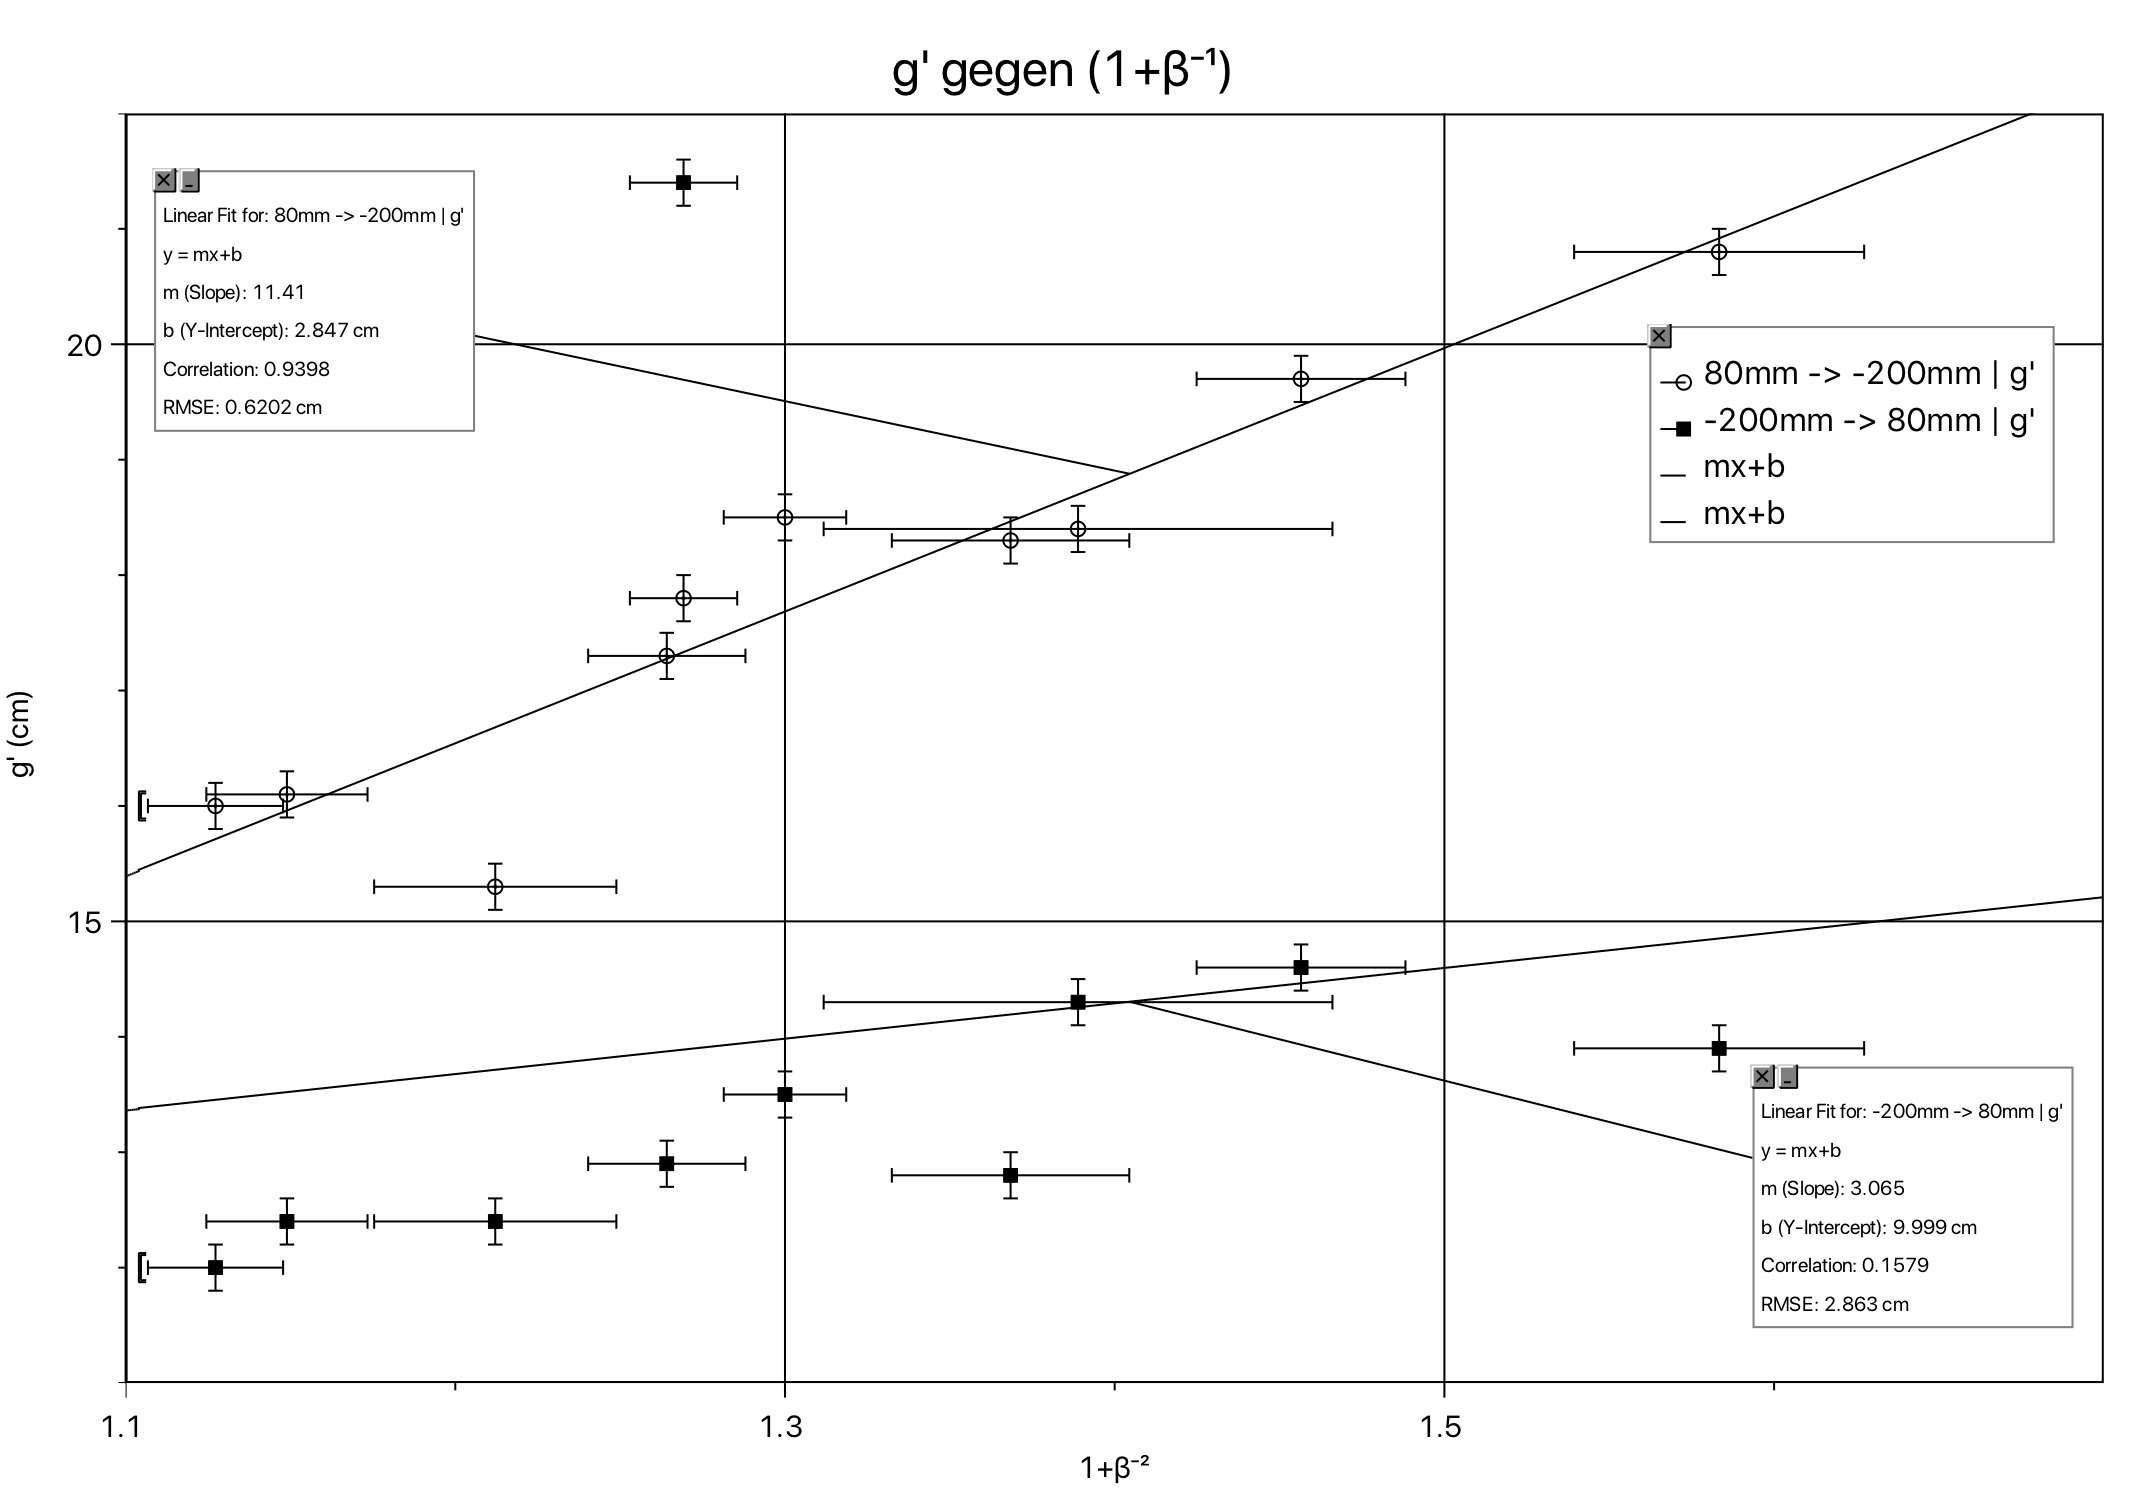
\includegraphics[width=\linewidth]{Abb4}
	\caption{Graph von $g'$ gegen $1+\frac{1}{\beta}$ für beide Linsensysteme}
\end{figure}

\begin{figure}[h]
	\centering
	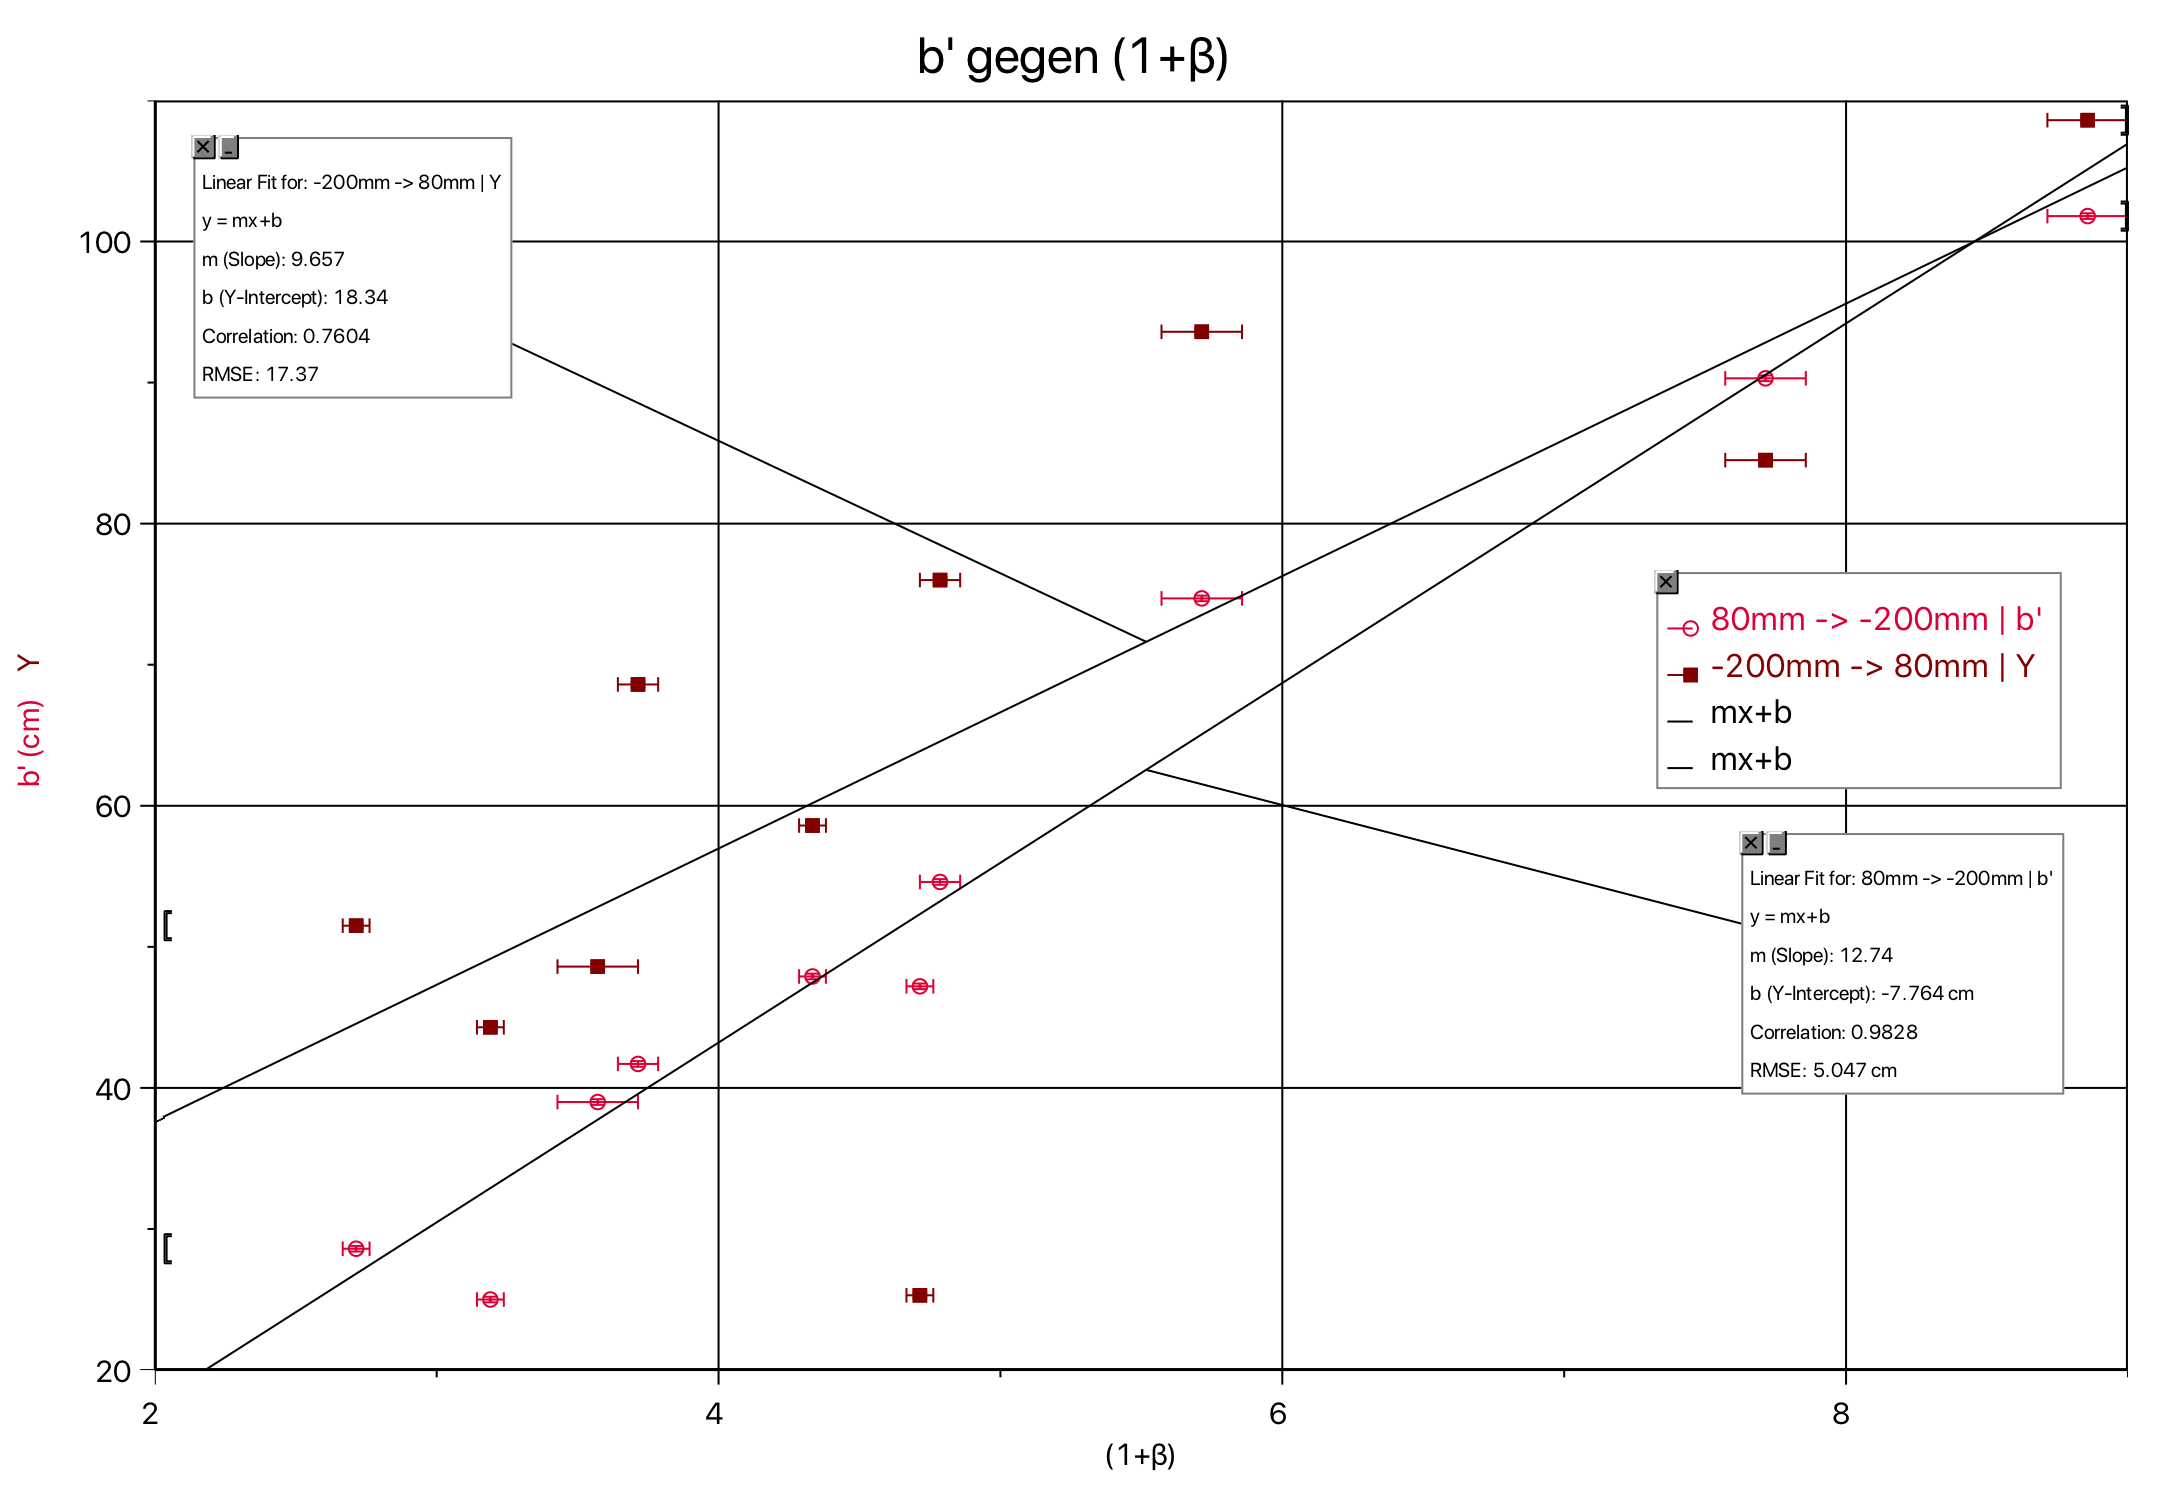
\includegraphics[width=\linewidth]{Abb5}
	\caption{Graph von $b'$ gegen $1+\beta$ für beide Linsensysteme}
\end{figure}

\end{document}